% ----------------------------------------------------------------------------
%                                Introduction
%-----------------------------------------------------------------------------
\newpage                                                 \chapter{Introduction}
\renewcommand{\thepage }{\arabic{page}}                    \setcounter{page}{1}

This paper focuses on the roles of audio and notifications generated by
intelligent agents within user interface design. It begins by reviewing previous
findings of HCI research where audio is used as \textit{the} primary element
of an interface as explored by Arons et al ~\cite{arons1991hyperspeech}. Attention is then
shifted to the work by Goose et al who used binaural audio as an interface for
HTML presentation ~\cite{goose19993dAudio}. Finally we explore a number of works
which have looked at binaural audio's role within interfaces incorporating other
modals ~\cite{ yu2006novel, marentakis2004study}.

Our work continues with the exploration of the role notifications have within
interface design. Experiments have shown that the impact of variable reliability
in a notification system biases users to ignore future notifications
~\cite{leetiernan2001effective}. This paper examines the  differences between
two types of notifications: informative ~\cite{maltz2000cue} and interpreted
~\cite{horvitz1999principles}. We also explore the effective and judicial use of
notification systems to inform future designs of our work~\cite{cutrell2001notification}.

The structure of this exploration is motivated by audible interfaces' ability to
provide an alternate mode of access to computers whenever a user's visual focus
is unavailable. Visual focus can be unavailable for a number of reasons, such as
when users are driving, using hand-held devices while engaged in other physical
activities that command your visual attention, or even as a result of physical
disabilities ~\cite{michelis2008disappearing}. There are a number of audible
interfaces which only provide a text-to-speech component allowing systems
to read the content of a visual interface to a user.  Text-to-speech solutions
often implement a monoaural speech pattern that provides a user with a single
channel of communication. Techniques exist to provide spatially placed (3D /
binaural) audio to listeners.  Our interest is in the use of spatial sound as
a main interface element for an audio interface.

%----------------------------------------------------------------------------%
\subsection{                 Motivation                                      }

T.V. Raman enumerated the differences between speech output interfaces and
screen reading solutions ~\citation{raman1996emacspeak}. He argued that the key
difference was the system's ability to give an application a voice (like
Emacspeak) versus simply reading a screen. Raman was introducing Emacspeak, an
application intended to give a voice to the terminal, not simply allowing a
machine to read what it is displaying. The precise difference he was making was
demonstrating that in creating Emacspeak as a subsystem of Emacs, Emacspeak had
context available to it that many screen readers simply cannot duplicate
~\cite{raman1996emacspeak}.

To this effect, our project researches how binaural audio and notification theory
can be combined to create new user interface designs. Our paper begins to lay the
foundation for future work by studying the roles of four particular combinations
of speech (ambient versus direct) and intelligent agent notifications (purely
informative versus interpretive). With our work we are exploring the ways in which
sound and notifications can be combined by different types of intelligent agents
to create interfaces with differing goals. We will explore the benefits of context
aware interfaces and the impact vocalization has on multi-tasking environments.


We motivate our work by using a common scenario like driving to work on a typical
morning. Eric Horvitz described how intelligent interfaces could be utilized to identify
what type of notifications to present in these situations ~\cite{horvitz1999principles}.
Some problems explored by Horvitz included what type of notifications a system should
use when an event occurs given the user's context.  In his work, Horvitz explored the
mechanisms that some systems could use to infer the types of actions specific events
may require. After inference, systems could provide notifications that offer to
automatically complete those actions.  A typical system of interest to us focuses
on the computer powering the navigation system in the previous scenario. While the
computer is providing navigation, it is also checking current road conditions
relative to the user's location. A connected smartphone has resumed polling work
email, the user's calendar has been updated by a colleague, and the user's
family is messaging them with a reminder for a prior engagement.  Each type stimulus
requires a stochastic decision that must be made regarding both the best method and
the proper time to alert the user. In his work, Horvitz quantified
the risks and benefits of using different notification paradigms to express this
information ~\cite{horvitz1999principles}. We explore how these trade offs present
themselves in the auditory domain.

%----------------------------------------------------------------------------%
\subsection{                 Project                                         }

We describe a system that supports a new conceptual model which maps interface
elements into a 3D audio space. Using binaural audio as the mechanism, novel
features are explored that provide information to the user in terms of spatial
attenuation, audio structural survey of content on the web, accurate positional
audio feedback and an audible progress indicator. These new features may improve
both the users' comprehension of content presented to them while providing users
with cues to assist in the recall of information.

Human auditory localization has been studied extensively~\cite{
yost1987directional, blauert1997spatial }. Because humans are especially adept
at localizing sounds in three dimensions we want to explore how predominant
auditory cues for determining whether a sound is coming from the left or right
directions can be used to portray other types of information.

The directional dependent filtering to each of a subject's ears can be expressed
as a frequency response, called a head related transfer function (HRTF), and
thus a pair of HRTFs describe how sound from one location reaches the two ears.
HRTFs are usually measured using human subjects or dummy-head microphones which
consist of response pairs for the left an right ears corresponding to a large
number of source positions surrounding the head. This will be the mechanism
powering the spatialization of this interface.

\begin{figure}[h]
  \centering
  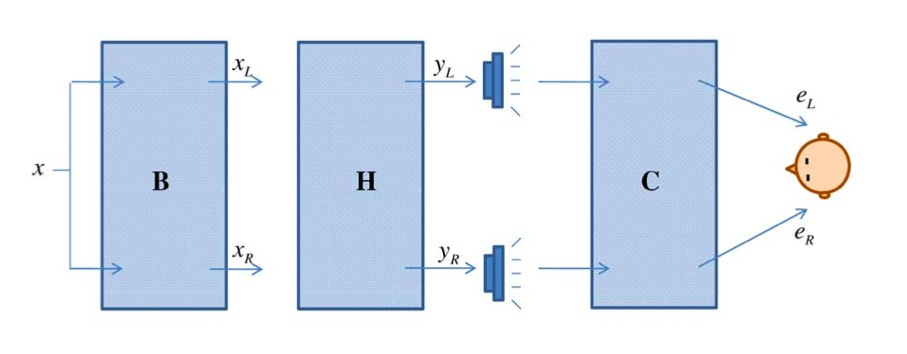
\includegraphics[width=1\textwidth]{images/binaural_diagram.jpg}
  \caption{Schematic of a binaural audio system}
\end{figure}

This thesis begins explore questions of efficiency of different types of intelligent
agents and how auditory interfaces can be used to better present multi-tasking
computing environments. While exploring the research in the utilization of audible
interfaces, this paper works towards two major goals. First a review of the prior
methodologies, processes, and terms necessary to study audible interfaces is
presented. In conjunction with this, an argument for the benefit of a 3D audio
interface will be presented as it applies to accessible solutions for users with
visual disabilities as well as the use by non-impaired users. In both cases, there
is an overlap in the needs of each user as vision either is not available or not
desired to be used as the primary interface with the system.

%-------------------------- where we're going --------------------------------%

A general background of binaural audio and audible interfaces are provided in
the following section. The related work connects ideas and findings both in the
fields of Human Computer Interaction and Artificial Intelligence to form the
basis for our approach in section 6. Finally, this work concludes with an
overview and survey of future work necessary for the creation of a binaural
audio interface as well as goals research in this area could pursue.
